\chapter[Background]{Background} \label{ch:bg}

% https://en.wikipedia.org/wiki/Quantum_computing
% https://en.wikipedia.org/wiki/Quantum_circuit
% https://en.wikipedia.org/wiki/Quantum_logic_gate

To understand quantum circuit optimization in the ZX-calculus, one first must understand quantum circuits and the ZX-calculus.
In this section we provide the requisite background in both of these, preceded by a brief discussion on qubits.
We conclude this section with an overview of quantum circuit optimization in the ZX-calculus.

\section{Qubits}\label{sec:qubits}

A classical bit has a value of 0 or 1.
A quantum bit, or \emph{qubit}, encodes a quantum superposition of these two values and therefore more information than a classical bit.
In the traditional bra-ket notation of quantum mechanics, a qubit is represented by a vector in $\mathbb{C}^2$,
\begin{align*}
  |\psi\rangle = \lambda_1 |0\rangle + \lambda_2 |1\rangle = \begin{pmatrix}\lambda_1 \\ \lambda_2 \end{pmatrix}
\end{align*}
where
\begin{align*}
  & |0\rangle = \begin{pmatrix}1 \\ 0\end{pmatrix} \\
  & |1\rangle = \begin{pmatrix}0 \\ 1\end{pmatrix}
\end{align*}
and $\lambda_1$ and $\lambda_2$ are the probability amplitudes of observing $|0\rangle$ and $|1\rangle$ upon measurement in this basis, respectively.
Notably, qubits can be written with respect to any orthonormal basis.
The set $\{|0\rangle, |1\rangle\}$ is known as the \emph{computational} basis.
Another common basis is the +/- basis, where
\begin{align*}
  & |+\rangle = \frac{|0\rangle + |1\rangle}{\sqrt{2}} \\
  & |-\rangle = \frac{|0\rangle - |1\rangle}{\sqrt{2}}
\end{align*}
The computational and +/- bases are also known as the Z and X bases, respectively.

More generally, a system of $n$ qubits is represented by the tensor product of the individual states.
So, an $n$-qubit state corresponds to a $2^{n}$-dimensional vector.
For example, the two-qubit state with both qubits in $|0\rangle$ is
\begin{align*}
  |0\rangle \otimes |0\rangle = |00\rangle = \begin{pmatrix}1 \\ 0 \\ 0 \\ 0\end{pmatrix}
\end{align*}
In the ZX-calculus and this work, qubits are abstracted as wires in string diagrams.
However, this definition is included both for completeness and to aid understanding of quantum circuits.

\begin{figure}
\centering
\begin{subfigure}{.5\textwidth}
  \centering
  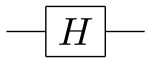
\includegraphics[width=.4\linewidth]{img/had}
  \caption{The Hadamard gate.}
  \label{fig:had}
\end{subfigure}%
\begin{subfigure}{.5\textwidth}
  \centering
  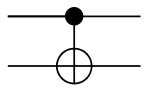
\includegraphics[width=.4\linewidth]{img/cnot}
  \caption{The CNOT gate. The top and bottom qubits are the control and target, respectively.}
  \label{fig:cnot}
\end{subfigure}
\caption{
  The circuit representation of two common quantum logic gates.
  Wires represent qubits and boxes represent quantum logic gates.
  Quantum circuits are read from left to right.
}
\label{fig:test}
\end{figure}


\section{Quantum Circuits}\label{sec:qcircs}

A quantum circuit models a quantum computation as a sequence of discrete gates.
In the traditional notation with qubits as vectors in $\mathbb{C}^2$, quantum gates correspond to unitary matrices.
For example, the Hadamard gate, a quantum gate that acts on a single qubit and maps
\begin{align*}
  & |0\rangle \mapsto \frac{|0\rangle + |1\rangle}{\sqrt{2}} \\
  & |1\rangle \mapsto \frac{|0\rangle - |1\rangle}{\sqrt{2}}
\end{align*}
has the matrix form
\begin{align*}
  H = \frac{1}{\sqrt{2}}\begin{bmatrix}1 & 1 \\ 1 & -1\end{bmatrix}
\end{align*}
Figure \ref{fig:had} depicts the circuit representation of the Hadamard gate.
Note that $|+\rangle = H|0\rangle$ and $|-\rangle = H|1\rangle$.
An important family of single-qubit gates are the \emph{phase shift} gates that modify the phase of the quantum state by some $\alpha$.
A phase shift gate maps
\begin{align*}
  & |0\rangle \mapsto |0\rangle \\
  & |1\rangle \mapsto e^{i\alpha}|1\rangle \\
\end{align*}
and has the matrix form
\begin{align*}
  R_{\alpha} = \begin{bmatrix}1 & 0 \\ 0 & e^{i\alpha}\end{bmatrix}
\end{align*}
Examples of phase gates are the T-gate ($\alpha = \frac{\pi}{4}$) and the S-gate ($\alpha = \frac{\pi}{2}$).
Phase gates where $\alpha$ is a multiple of $\pi / 2$ are called \emph{Clifford} gates.

Quantum gates are not restricted to acting on single qubits.
For example, the controlled-NOT (CNOT) gate acts on two qubits and flips the second (target) qubit only when the first (control) qubit is $|1\rangle$.
The CNOT gate is typically depicted as shown in Figure \ref{fig:cnot} and has the following matrix form:
\begin{align*}
  CNOT = \begin{bmatrix}1 & 0 & 0 & 0 \\0 & 1 & 0 & 0 \\ 0 & 0 & 0 & 1\\0 & 0 & 1 & 0\end{bmatrix}
\end{align*}
In general, an $n$-qubit gate is represented by a $2^n$-dimensional unitary.
However, attention is typically restricted to single- and 2-qubit gates as it is well known that the Clifford + T gate set, consisting of the H, T, S, and CNOT gates, is \emph{universal} -- any other operation can be represented by a finite sequence from this set.
The \emph{Clifford circuits} are those that can be generated by $\{H, S, CNOT\}$.
As the T and S gates are instances of phase shift gates, $\{H, R_{\alpha}, CNOT\}$ is also universal though in practice any non-Clifford phase gate is implemented with T gates. % FIXME: Is this true?
% A subset of all operators, \emph{Clifford circuits} are those that can be generated by $\{H, S, CNOT\}$ (i.e., by fixing $\alpha = \pi / 2$).

Quantum gates can be composed sequentially or in parallel.
Consider two gates $A$ and $B$.
The effect of $B$ applied in series after $A$ can be described by a single gate (i.e., linear map) via matrix multiplication (i.e., $B \cdot A$).
Alternatively, the tensor product is used to describe A and B in parallel (i.e., $B \otimes A$).
For example, the simple circuit shown in Figure \ref{fig:simple-trad} can be described by the following linear map:
\begin{align*}
  (\mathbb{I} \otimes CNOT) \cdot (\mathbb{I} \otimes H \otimes \mathbb{I}) \cdot (CNOT \otimes \mathbb{I}) \cdot (S \otimes \mathbb{I} \otimes \mathbb{I})
\end{align*}



\begin{figure}
\centering
\tikzfig{ZX-rules}
\caption{
  The rules of the ZX-calculus.
  All rules hold with the colors interchanged and for $\alpha, \beta \in [0, 2 \pi)$.}
\label{fig:zx-rules}
\end{figure}



\section{ZX-Calculus}\label{sec:zx}

The ZX-calculus is a graphical language for representing and reasoning about quantum processes.
Quantum processes are represented by \emph{ZX-diagrams} which consist of \emph{wires} and \emph{spiders}.
Spiders can have an arbitrary number of inputs and outputs and come in two flavors: Z spiders (shown in green) and X spiders (shown in red).
As with quantum circuits, a ZX-diagram is interpreted from left to right.

ZX-diagrams abstract away the complexities of linear algebra and tensor products from traditional formalisms of quantum processes.
Wires still represent qubits while spiders provide a general form for linear maps, where
\begin{align*}
  & \tikzfig{Zsp-a} := \ketbra{0...0}{0...0} + e^{i\alpha}\ketbra{1...1}{1...1} \\
  & \tikzfig{Xsp-a} := \ketbra{+...+}{+...+} + e^{i\alpha}\ketbra{-...-}{-...-}
\end{align*}
Two diagrams can be composed in serial by joining the outputs of the first to the inputs of the second, or in parallel by stacking the two diagrams.

From this definition, we can identify the diagrammatic represenations for several common components of quantum computation:
\[
\begin{array}{rclcrcl}
\tikzfig{ket-+} & = & \ket{0} + \ket{1} \ \propto \ket{+} &
\qquad\qquad &
\tikzfig{ket-0} & = & \ket{+} + \ket{-} \ \propto \ket{0} \\
&\quad& & & \quad \\
\tikzfig{Z} & = & \ketbra{0}{0} - \ketbra{1}{1} = Z &
&
\tikzfig{X} & = & \ketbra{+}{+} - \ketbra{-}{-} = X
\end{array}
\]
where $Z$ and $X$ are the corresponding Pauli matrices.
Note that spiders without any inputs can be regarded as qubit state preparations.
The Hadamard gate is so pervasive that it merits shorthand notation;
we use a yellow square to represent the Hadamard gate as shown below
% \ctikzfig{had-alt}
\begin{equation}\label{eq:had-short}
  \tikzfig{had-alt}
\end{equation}
and replace a Hadamard gate between two spiders with a blue dashed edge:
\ctikzfig{blue-edge-def}

We can also reason about ZX-diagrams.
The first rule for determining equality is that \emph{only connectivity matters} (OCM).
In other words, two ZX-diagrams are equal when one can be deformed into the other (e.g., via moving vertices around in the plane or bending wires) while maintaining connectivity and the order of the inputs and outputs.
In addition to this OCM principle, the ZX-calculus includes a primary set of rewrite rules as shown in Figure \ref{fig:zx-rules}.
These rules only hold up to non-zero scalar factors, though these scalars are typically ignored as they correspond to negligible differences in global phase.
Additional rules can be derived from this set, such as the antipode rule
\ctikzfig{hopf-rule}
and the $\pi$-copy rule
\ctikzfig{picopy-rule}

All quantum circuits can be translated to ZX-diagrams.
This is a consequence of the fact that the following universal gate set can be easily represented in the ZX-calculus:
\begin{align*}
CNOT & = \tikzfig{cnot} &
R_{\alpha} & = \tikzfig{Z-a} &
H & = \tikzfig{h-alone}
\end{align*}
In the CNOT diagram, the green and red spiders are the control and target qubits, respectively.
As an example, Figure \ref{fig:simple-circ} depicts both the traditional and diagrammatic representations of a simple quantum circuit.



\begin{figure}
\centering
\begin{subfigure}[t]{.3\textwidth}
  \centering
  % 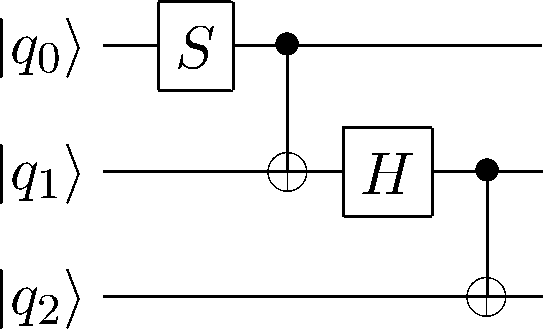
\includegraphics[width=.4\linewidth]{img/traditional.png}
  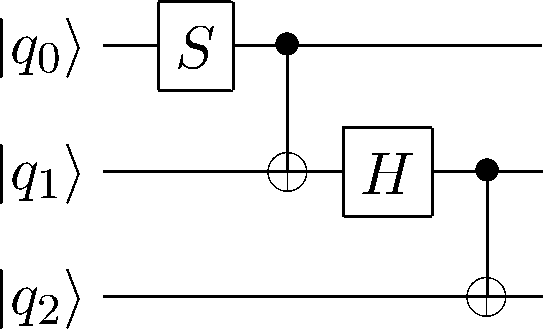
\includegraphics[width=4cm]{img/traditional.png}
  \caption{Traditional notation}
  \label{fig:simple-trad}
\end{subfigure}%
\begin{subfigure}[t]{.7\textwidth}
  \centering
  \resizebox{9cm}{!}{\begin{tikzpicture}
	\begin{pgfonlayer}{nodelayer}
		\node [style=none] (0) at (-5.75, 1) {};
		\node [style=none] (1) at (-5.75, 0) {};
		\node [style=none] (2) at (-5.75, -1) {};
		\node [style=Z phase dot] (3) at (-4.75, 1) {$\frac{\pi}{2}$};
		\node [style=X dot] (4) at (-3.75, 0) {};
		\node [style=Z dot] (5) at (-3.75, 1) {};
		\node [style=Z dot] (6) at (-2.75, 0) {};
		\node [style=X dot] (7) at (-1.75, -1) {};
		\node [style=Z dot] (8) at (-1.75, 0) {};
		\node [style=none] (9) at (-0.75, 1) {};
		\node [style=none] (10) at (-0.75, 0) {};
		\node [style=none] (11) at (-0.75, -1) {};
		\node [style=none] (12) at (0.75, 1) {};
		\node [style=none] (13) at (0.75, 0) {};
		\node [style=none] (14) at (0.75, -1) {};
		\node [style=Z phase dot] (15) at (1.75, 1) {$\frac{\pi}{2}$};
		\node [style=X dot] (16) at (1.75, 0) {};
		\node [style=Z dot] (17) at (2.75, 0) {};
		\node [style=X dot] (18) at (2.75, -1) {};
		\node [style=none] (19) at (3.75, 1) {};
		\node [style=none] (20) at (3.75, 0) {};
		\node [style=none] (21) at (3.75, -1) {};
		\node [style=none] (22) at (0, 0) {=};
	\end{pgfonlayer}
	\begin{pgfonlayer}{edgelayer}
		\draw (0.center) to (3);
		\draw (1.center) to (4);
		\draw (2.center) to (7);
		\draw (3) to (5);
		\draw (4) to (5);
		\draw [style=hadamard edge] (4) to (6);
		\draw (5) to (9.center);
		\draw (6) to (8);
		\draw (7) to (8);
		\draw (7) to (11.center);
		\draw (8) to (10.center);
		\draw (12.center) to (15);
		\draw (13.center) to (16);
		\draw (14.center) to (18);
		\draw (15) to (16);
		\draw (15) to (19.center);
		\draw [style=hadamard edge] (16) to (17);
		\draw (17) to (18);
		\draw (17) to (20.center);
		\draw (18) to (21.center);
	\end{pgfonlayer}
\end{tikzpicture}
}
  \caption{ZX-diagram}
  \label{fig:simple-zx}
\end{subfigure}
\caption{A simple 3-qubit quantum circuit shown in both the traditional notation and as a ZX-diagram.}
\label{fig:simple-circ}
\end{figure}


\section{Circuit Optimization in the ZX-Calculus}\label{sec:zx-circ-opt}

% Note: be careful about circuit-like graph. This is stricter than circuit-extractability (from_graph vs. extract_circuit

The goal of quantum circuit optimization is to simplify quantum circuits (e.g., via reducing the number of gates) to reduce noise and decoherence when run on modern quantum computers.
More specifically, the T-count and 2-qubit-count are typically targeted; fault tolerant implementations of T gates generally require an order of magnitude more resources than Clifford gates~\cite{campbell2017roads}, and the fidelity of single-qubit gates is demonstrably higher than that of 2-qubit gates~\cite{ballance2016high}.
It is standard to perform optimizations at the circuit-level.
Examples of circuit-level optimizations are 3-qubit gate decomposition and cancelling back-to-back CNOT gates.

The ZX-calculus enables circuit optimization at the graph-level, a more flexible setting that is well-studied in its own right.
Such an optimization involves converting a circuit to a ZX-diagram, simplifying the diagram, and converting the diagram back to a circuit. % TODO: Could have a figure for this pipeline
However, there is no known general-purpose procedure for recovering a quantum circuit from a generic ZX-diagram.
This restricts the space of permissible simplifications to those that preserve whichever diagrammatic properties are required by the extraction procedure.


\begin{figure}
\centering
\tikzfig{graph-like-ex}
\caption{An example of a ZX-diagram and an equivalent, graph-like ZX-diagram.}
\label{fig:graph-like}
\end{figure}

In 2020, Duncan et al. reported an extraction procedure that enabled current best practices~\cite{duncan2020graph}.
Firstly, this procedure operates on \emph{graph-like} ZX-diagrams.
A ZX-diagram is graph-like when:
\begin{enumerate}
\item
  All spiders are Z-spiders.
\item
  Z-spiders are only connected via Hadamard edges
\item
  There are no parallel Hadamard edges or self-loops
\item
  Every input or output is connected to a Z-spider and every Z-spider is connected to at most one input or output
\end{enumerate}
Every ZX-diagram is equal to a graph-like diagram (see Figure \ref{fig:graph-like} for an example), and this form admits an underlying graph structure that permits graph-theoretic analyses.
Secondly, this procedure requires that the underlying graph of the input ZX-diagram satisfies a graph-theoretic invariant called \emph{focused generalized flow} (focused gFlow). % which guarantees that FIXME.
Given such an input ZX-diagram, extraction proceeds in such a way that each non-zero phase corresponds to one phase gate in the resulting circuit but each edge can correspond to multiple CNOTs.
For this reason, local changes in a ZX-diagram (e.g., connectivity) can have significant effects on the complexity of the associated circuit.
Importantly, this extraction procedure is not optimal;
if a given circuit is converted to a ZX-diagram and the extraction procedure is immediately applied, the extracted circuit is often more complex than the original circuit.
In particular, this procedure can drastically increase the number of 2-qubit gates.
For more details on the extraction procedure or focused gFlow, see \cite{duncan2020graph}.

% Note: be careful. focused gFlow is something that exists. E.g., "The existence of a focused gFlow is preserved by local complementation and pivoting"

Alongside this extraction procedure, Duncan et al. also introduced an optimization procedure that relies on focused gFlow-preserving graph simplifications.
More specifically, this procedure relies on two graph-theoretic transformations that each correspond to rewrite rule in the ZX-calculus: \emph{local complementation} and \emph{pivoting}.
Given a graph $G$ and some vertex $u$ of $G$, the \emph{local complementation} of $G$ according to $u$, denoted $G \star u$, is the graph in which the connectivity of all pairs of neighbors of $u$ is inverted.
For example,
\begin{equation*}
G\quad\tikzfig{graph1-lab}\qquad\qquad G\star a\quad\tikzfig{graph1-lab-1}
\end{equation*}
Given a ZX-diagram, local complementation can be induced in the underlying graph structure while maintaining equality by applying an $X_{-\pi/2}$ gate on (the spider corresponding to) $u$ and a $Z_{\pi/2}$ gate to its neighbors~\cite{duncan2009graph}:
% \ctikzfig{local-comp-ex}
\begin{equation}\label{eq:gs-local-comp}
  \tikzfig{local-comp-ex}
\end{equation}
Relatedly, given two connected vertices $u$ and $v$ in $G$, the \emph{pivot} of $G$ along the edge $uv$ is the graph $G \wedge uv :=G \star u \star v \star u$.
In practice, this consists of complementing the edges between three subsets of vertices: (1) the common neighborhood of $u$ and $v$, (2) the exclusive neighborhood of $u$, and (3) the exclusive neighborhood of $v$:
\[G \quad\tikzfig{pivot-L}\qquad\qquad \quad G\wedge uv \quad\tikzfig{pivot-R}
\]
Again, given a ZX-diagram, the rewrite rule reported in \cite{duncan2013pivoting} introduces a pivot by applying Hadamard gates on $u$ and $v$ and $Z_{\pi}$ gates on their common neighborhood:
% \ctikzfig{pivot-desc}
\begin{equation}\label{eq:gs-pivot}
  \tikzfig{pivot-desc}
\end{equation}
Each rewrite rule can be extended to a simplification by performing local complementation (resp. pivoting), removing the vertex (resp. the pair of vertices), and updating the phases:
\ctikzfig{lc-simp}
\ctikzfig{pivot-simp}
Importantly, the existence of a focused gFlow is preserved in both cases.
At a high-level, optimization can then be performed by applying these simplifications to fixpoint and extracting a circuit from the resulting ZX-diagram.
Details on this optimization procedure and proofs of the simplification rules or their focused gFlow-preservation can be found in \cite{duncan2020graph}.
A variant of this procedure is implemented in the \codeword{full_reduce} method of the PyZX library.

One issue with \codeword{full_reduce} is its reliance on circuit extraction; it is not uncommon that the circuit extracted from the final, simplified ZX-diagram has more gates than the input circuit.
Kissinger and van de Wetering introduced an alternative optimization method that uses \emph{phase teleportation} to sidestep the issue of circuit extraction altogether~\cite{kissinger2019reducing}.
Crucially, simplification of the ZX-diagram is performed symbollically.
% In addition to the aforementioned rules, this procedure uses several new rewrite rules that remove interior Pauli spiders at the cost of introducing \emph{phase-gadgets}, a ZX-diagrammatic motif.
This symbolic simplification leverages the fact that several rewrite rules involving \emph{phase-gadgets}, a particular ZX-diagrammatic motif, correspond to changes in the original phases.
Therefore, non-Clifford phases can potentially cancel or combine with each other while leaving the original graphical structure of the ZX-diagram intact.
% By exploiting a particular motif, the \emph{phase-gadget}, particular rewrite rules correspond to changes in the phases of the original ZX-diagram.
% So, as simplification proceeds using both the aforementioned rules as well as several new rewrite rules (that remove interior Pauli spiders at the cost of introducing phase-gadgets), changes in the original diagram are simply tabulated, absolving the need for extraction.
So, as simplification proceeds, application of these rules is simply tabulated to enable reconstruction of a final circuit with the same connectivity but a possible reduction in non-Clifford gates (and therefore T-count).
% using both the rules described above as well as several new rewrite rules that remove any remaining interior Pauli spiders at the cost of introducing \emph{phase-gadgets}, a particular ZX-diagrammatic motif.
% Instead, the ZX-diagram is first simplified using both rules described above as well as several new rewrite rules that remove any remaining interior Pauli spiders at the cost of introducing \emph{phase-gadgets}, a particular ZX-diagrammatic motif.
Importantly, using phase teleportation rather than circuit extraction ensures that the number of 2-qubit and Hadamard gates is unchanged. % while the T-count can be reduced.
By changing the angles of many non-Clifford phase gates to either 0 or multiples of $\pi /2$, this procedure can also make a circuit-level optimization procedure much more effective.
% In this way, this simplification procedure never increases the number of 2-qubit or Hadamard gates and can only reduce T-count.
This procedure is implemented in the \codeword{teleport_reduce} method of PyZX.
% and gates are always paplied between the same pairs of qubits as before
% non-Clifford phases can potentially cancel or combine with each other
